%!TEX root = ../MasterThesis.tex

\section{Peer-to-peer communication}
\label{sec:p2p_communication}

This section explains the core concepts of \gls{P2P} communication technologies. It begins with a comparision of the benefits and disadvantages of centralized and decentralized Web architectures. After that it shows how \gls{P2P} communication networks can be structured, different ways to initiate a communication session as well as how data can be transmitted between peers.

\subsection{Centralized vs. Decentralized Web Architectures}
\label{sec:central_decentral_arch}

In classical client-server applications the information is stored on a central system (aka server). Clients have to connect to the server and ask for the information. The server handles the requests from the clients and deliver the information in case a request was valid. A prominent example of the client-server architecture is the World-Wide Web as it exists today, in which clients (in this case the Web browser running on a computer) is communicating with a Web server (running on a server of owner of a Web site) to access and retrieve Web documents (e.g.\ \gls{HTML}, images, audio, video, \ldots) transmitted via the \gls{HTTP} protocol, as shown in Figure~\ref{fig:p2p_central_server}. \@

\begin{figure}[H]
	\centering
		\includegraphics[width=0.9\columnwidth]{images/client-server-web.png}
	\caption[Client-Server communication as used on the World-Wide Web]{Client-Server communication as used on the World-Wide Web \citep{codeTuts}}
\label{fig:p2p_central_server}
\end{figure}

As a consequence of this architecture the information is centralized and under control of the provider of the (Web) server. This can lead to a variety of problems, including serious issues such as unreliable or no longer existing servers will result in a dismissal of all the information stored on them, or privacy concerns for user-generated content stored on those central servers. \\

In opposite to that a \gls{P2P} network considers all nodes as equal. This offers the benefit that information can be kept on each node, and each node can provide access to its information to any other node on the network. Due to this the \gls{P2P} system has an high degree of decentralization, is not owned and controlled by a specific company, and therefore tends to me more resilient to faults, outages and attacks. But due to the distributed nature of it looking for and accessing information is more difficult. Information in a \gls{P2P} system have to be indexed in a way so that the correct node is queried for it. Still this index has to be stored somewhere in the system, and the optimal solution for the indexing problem depends on the type of \gls{P2P} system used (see next section). Additionally, the way new nodes get connected to the system is depending on the type of \gls{P2P} system used, and might lead to the introduction of special bootstrap or super nodes into the system as shown in Figure~\ref{fig:p2p_overlay_network} \citep{parameswaran2001p2p}.

\begin{figure}[H]
	\centering
		\includegraphics[width=0.9\columnwidth]{images/p2p_network.png}
	\caption[A \gls{P2P} overlay network]{A \gls{P2P} overlay network \citep[pg. 9]{buford2009p2p}}
\label{fig:p2p_overlay_network}
\end{figure}

% section central_decentral_arch (end)

\subsection{Classification of \gls{P2P} systems}
\label{sec:p2p_classification}

\gls{P2P} system architectures can be classified based on their degree of centralization into: \@

\begin{itemize}
	\item \textbf{partially centralized \gls{P2P} system:} rely on a dedicated controller node that maintains the set of participating nodes, host the index of the information available in the system, and controls the overall operation of the network,
	\item \textbf{decentralized \gls{P2P} system:} does not use any dedicated controller node, but may need to introduce bootstrap and super nodes for maintaining the list of participating nodes and the index of the information available depending on the size of the network.
\end{itemize}

% section p2p_classification (end)

\subsection{Communication in a \gls{P2P} communication}
\label{sec:p2p_start_communication}

The procedure to establish a \gls{P2P} communication depends on the structure of the \gls{P2P} system. In a \emph{partly centralized \gls{P2P} system} new nodes join the network by connecting to the central controller first. This central controller has a well-known \gls{IP} address and maintains the operation of the whole \gls{P2P} network. Due to this, any new node has to register with the central controller to get introduced to the \gls{P2P} network. The controller also maintains the information about the overlay network as well as the information about each object and on which node(s) it resides within the network. The overlay is typically following a star-shaped topology with the central controller at the center, see Figure~\ref{fig:p2p_network_structures}. \\

In a \emph{decentralized \gls{P2P} system} new nodes are expected to obtain the \gls{IP} address they have to connect to initially via a separate channel (e.g.\ as a link on a Web site). Depending on the size of the \gls{P2P} network additional bootstrap or super nodes, which help to set up a new node, are available on the network. These special nodes are generally also consolidating information about the objects available on the peers nearby, which helps speeding up searching and accessing required information. The overlay information of such distributed network can be either \emph{structured}, in which each node receives a unique identifier from a numeric keyspace resembling the responsibilities of that node, or \emph{unstructured}, in which there no particular structure or constraints assigned to the nodes of the network. \\

A \emph{structured overlay} maintain the information within the network more efficiently, because it uses a distributed hash-table to maintain a distributed index and decides the location (aka node) of an object in the network based on its hash-value. In an \emph{unstructured overlay network} the information is typically stored on the node that introduces it. To locate an object a query request is typically broadcasted through the overlay network. Based on the size of the network and the distance between the node asking for the information and the node holding the information querying and accessing an information on an unstructured overlay network will take time, and can also flood the whole network with query requests. Therefore, requesting nodes often set the scope of the request, which limits the number of hops that should be done on the network. This will reduce the overhead on the whole system. Additionally, introducing super nodes that collect and maintain indexes of their peers nearby can further reduce the number of hops necessary to find the required information, see Figure~\ref{fig:p2p_network_structures} \citep{rodrigues2010peer}. \@

\begin{figure}[H]
	\centering
		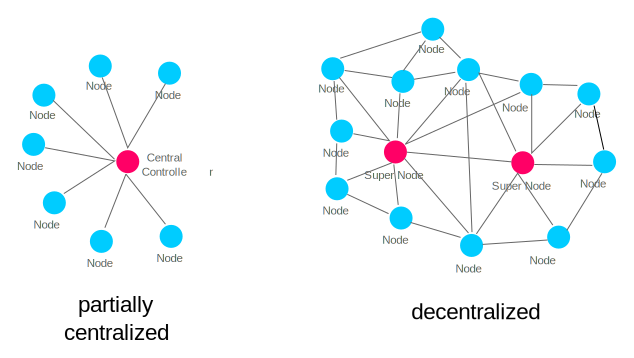
\includegraphics[width=0.8\columnwidth]{images/p2p_network_structures.pdf}
	\caption{Possible \gls{P2P} network structures}
\label{fig:p2p_network_structures}
\end{figure}

% section p2p_start_communication

\subsection{\gls{WebRTC} protocol}
\label{sec:p2p_webrtc}


% section p2p_webrtc (end)

% section p2p_communication (end)
